\thispagestyle{empty}\SourceLeaf{2}
\pdfbookmark[0]{Carl Friedrich Gauss, Works. Volume V}{volume-title}
\vspace*{1.8in}
\begin{center}
{\fontsize{18}{23}\selectfont CARL FRIEDRICH GAUSS WORKS\par}
\vspace{.5in}
{\Large VOLUME V.\par}
\end{center}
\clearpage
\thispagestyle{empty}\SourceLeaf{4}
\begin{center}
{\Large CARL FRIEDRICH GAUSS\par}
\vspace{.3in}
{\Huge WORKS\par}
\vspace{.3in}
{\large FIFTH VOLUME\par}
\vspace{.35in}
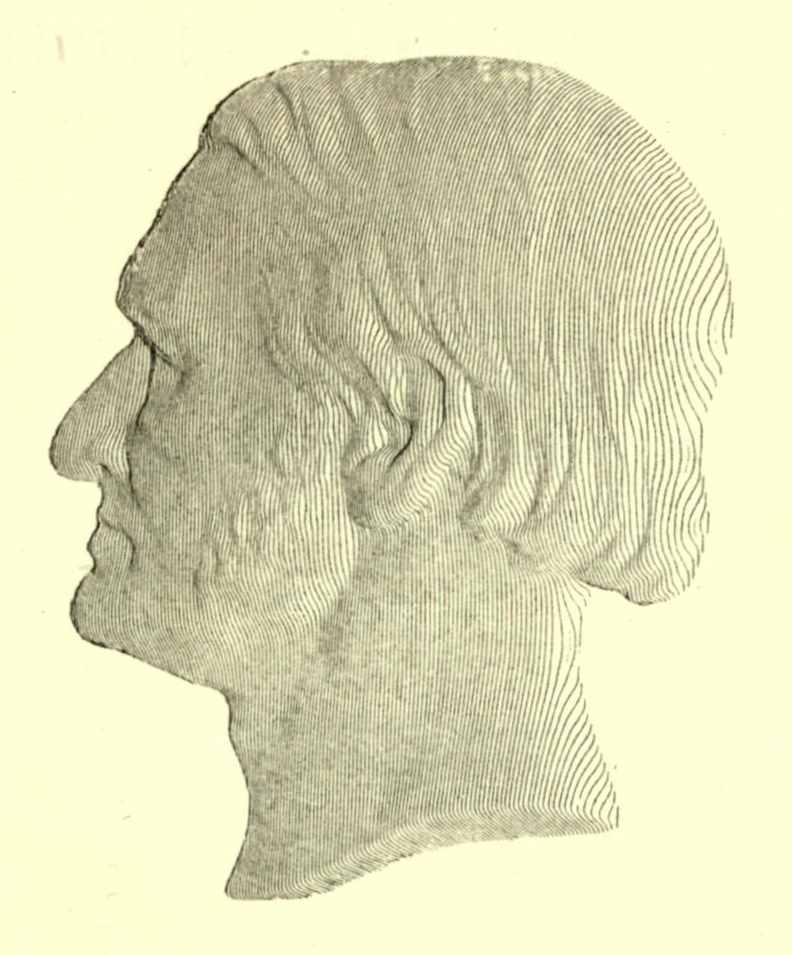
\includegraphics[height=2.2in]{figures/gauss_portrait_native004.png}\par
\vspace{.35in}
{\normalsize EDITED\par}
\medskip
{\small BY THE\par}
\medskip
{\normalsize ROYAL SOCIETY OF SCIENCES\par}
\medskip
{\small AT\par}
\medskip
{\Large GÖTTINGEN\par}
\medskip
{\large 1867.\par}
\end{center}
\clearpage
\thispagestyle{empty}\SourceLeaf{5}
\pdfbookmark[0]{Theory of attraction. Title}{attractionis-title}
\begin{center}
\vspace*{.45in}
{\large THEORY OF THE ATTRACTION OF\par}
\bigskip
{\Large HOMOGENEOUS ELLIPTIC\par}
\bigskip
{\large SPHEROIDAL BODIES\par}
\bigskip
{\normalsize TREATED BY A NEW METHOD\par}
\vspace{.5in}
{\small BY\par}
\vspace{.5in}
{\large CARL FRIEDRICH GAUSS\par}
\vspace{.55in}
{\small PRESENTED TO THE ROYAL SOCIETY OF SCIENCES ON 18 MARCH 1813.\par}
\vfill
\rule{.8\textwidth}{.3pt}\par
\medskip
{\small Commentationes societatis regiae scientiarum Gottingensis recentiores. Vol.~\textsc{ii}\par}
\smallskip
Göttingen \textsc{mdcccxiii}.\par
\medskip
\rule{.8\textwidth}{.3pt}\par
\end{center}
\clearpage
